% !TeX root = ../main.tex

\chapter{基于深度学习的时间序列异常检测框架设计与实现}
\label{cha:intro}
本章主要介绍本文实现的基于深度学习的时间序列异常检测框架,对执行流程和各个部分的设计进行详细说明。
\section{形式化定义}
首先我们形式化地描述一下时间序列异常检测问题。一个时间序列是等时间间隔收集到的各个指标的值,定义为${\rm x}=\{{\rm x}_1,{\rm x}_2,\dots,{\rm x}_N\}$,$N$是收集的次数。由于本文考虑的是多元时间序列的异常检测,所以每个时间都会有多个监测指标的值,也就是其中${\rm x}_t\in R^M$,${\rm x}_t=[x_t^1,x_t^2,\dots,x_t^M]$,其中$t\leq N$,$M$是数据的维度。所以${\rm x}\in R^{N\times M}$。我们最终目标是输出一个$y=[y_1, y_2,\dots, y_N ]$,其中$y_t\in \{0,1\}$,$y_t=0$代表该时刻检测到的指标正常,否则认为发现一个异常。图\ref{fig:anomaly_example}展示了一个异常。
\begin{figure}[htbp]
  \centering
  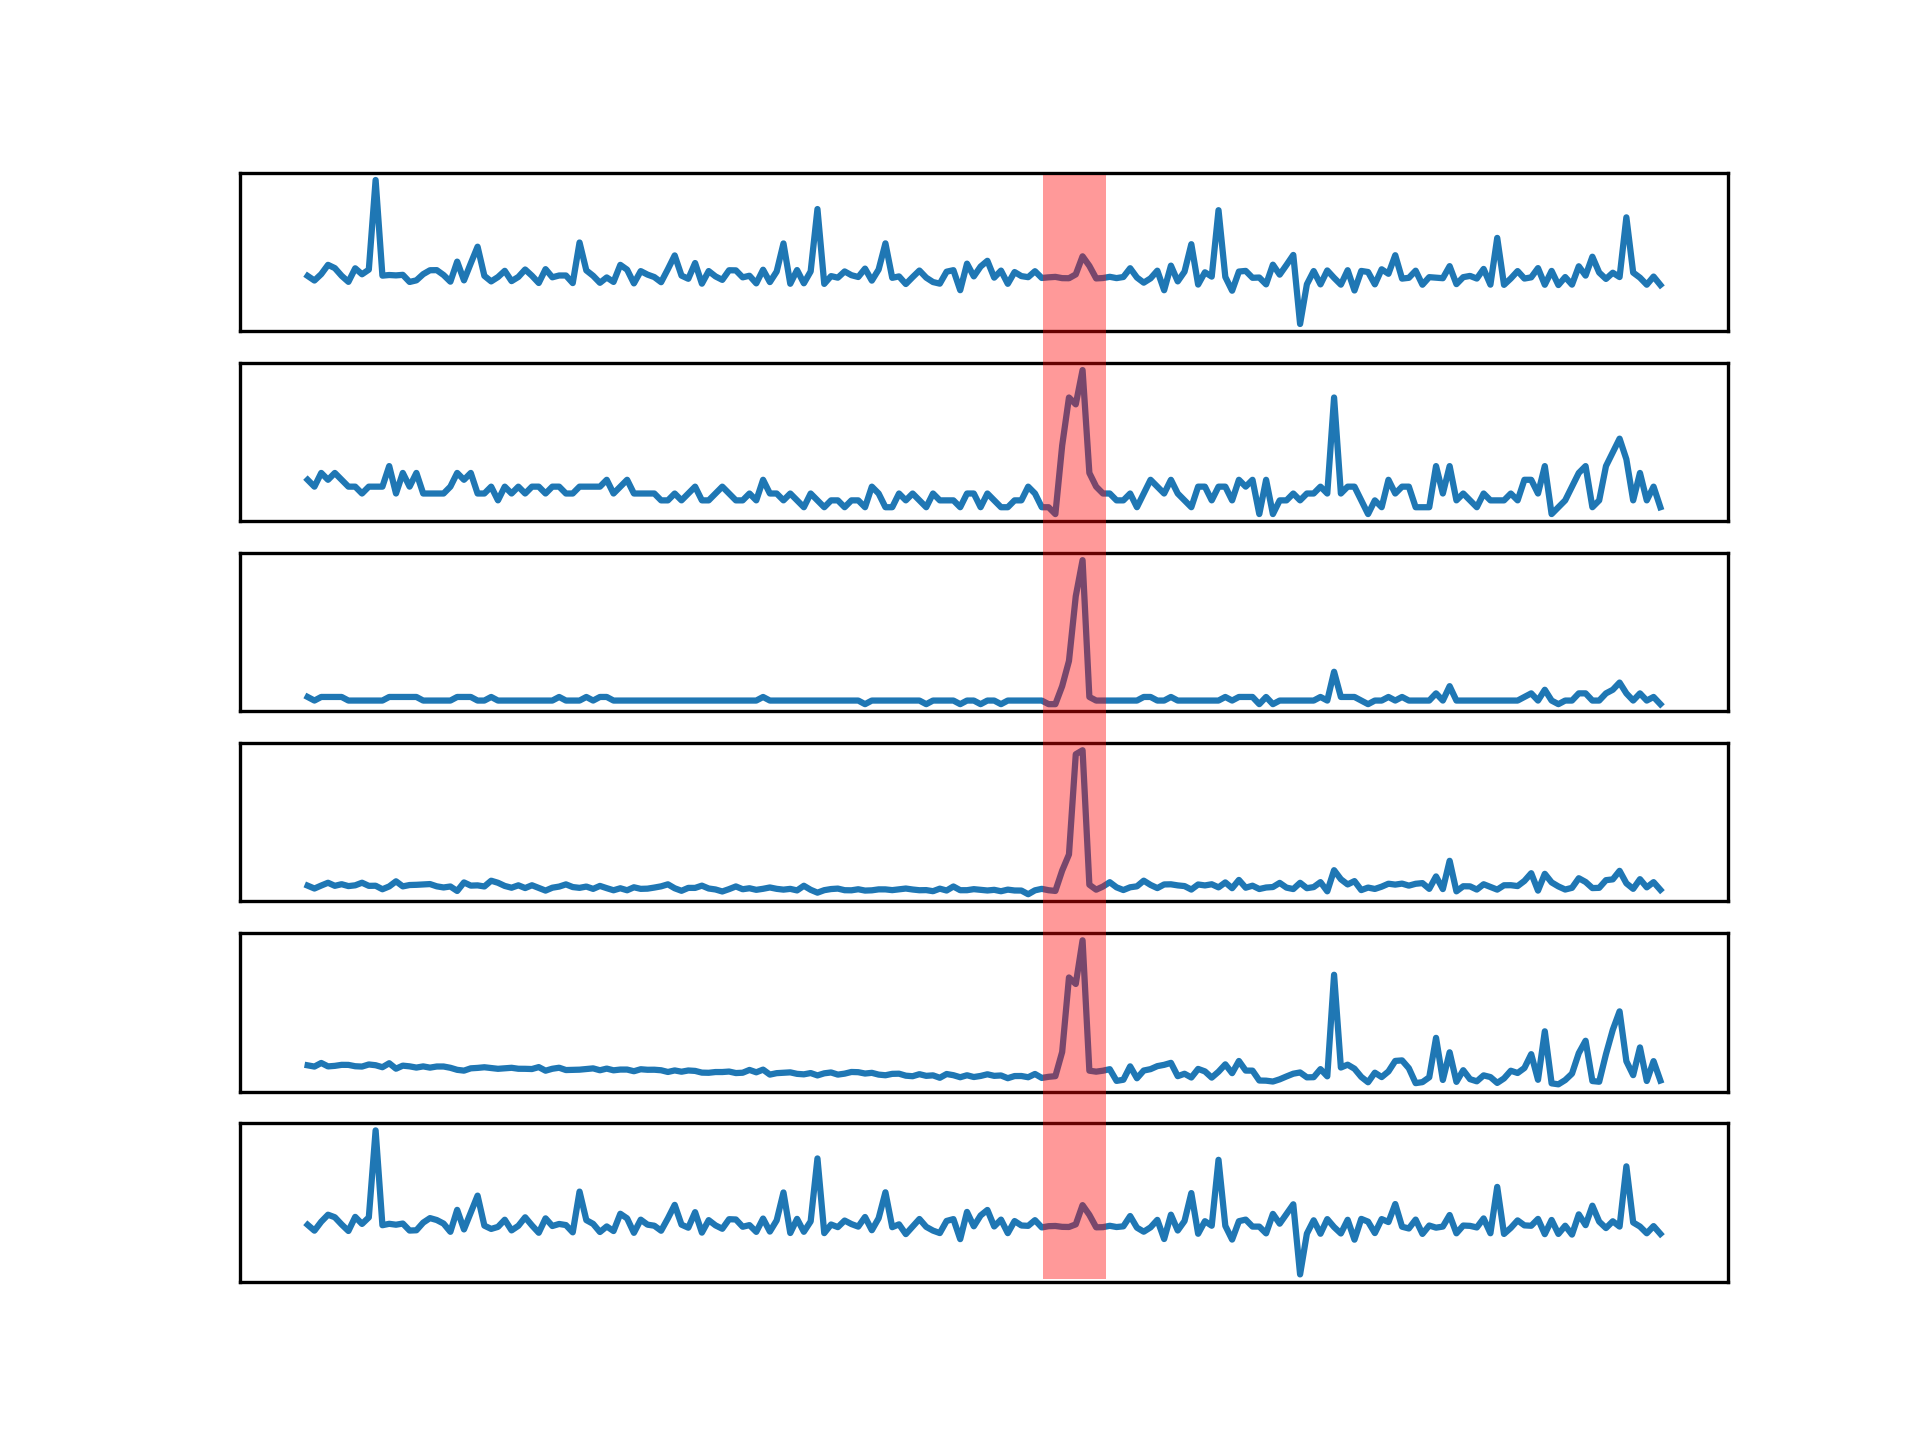
\includegraphics[width=\textwidth]{another_anomaly_example.png}
  \caption{多维时间序列数据中的一个异常示例,其中标红部分为一个异常}
  \label{fig:anomaly_example}
\end{figure}

\section{框架设计}
本文实现的基于深度学习的时间序列异常检测框架如图~\ref{fig:part1_overview}所示

\begin{figure}[htbp]
    \centering
    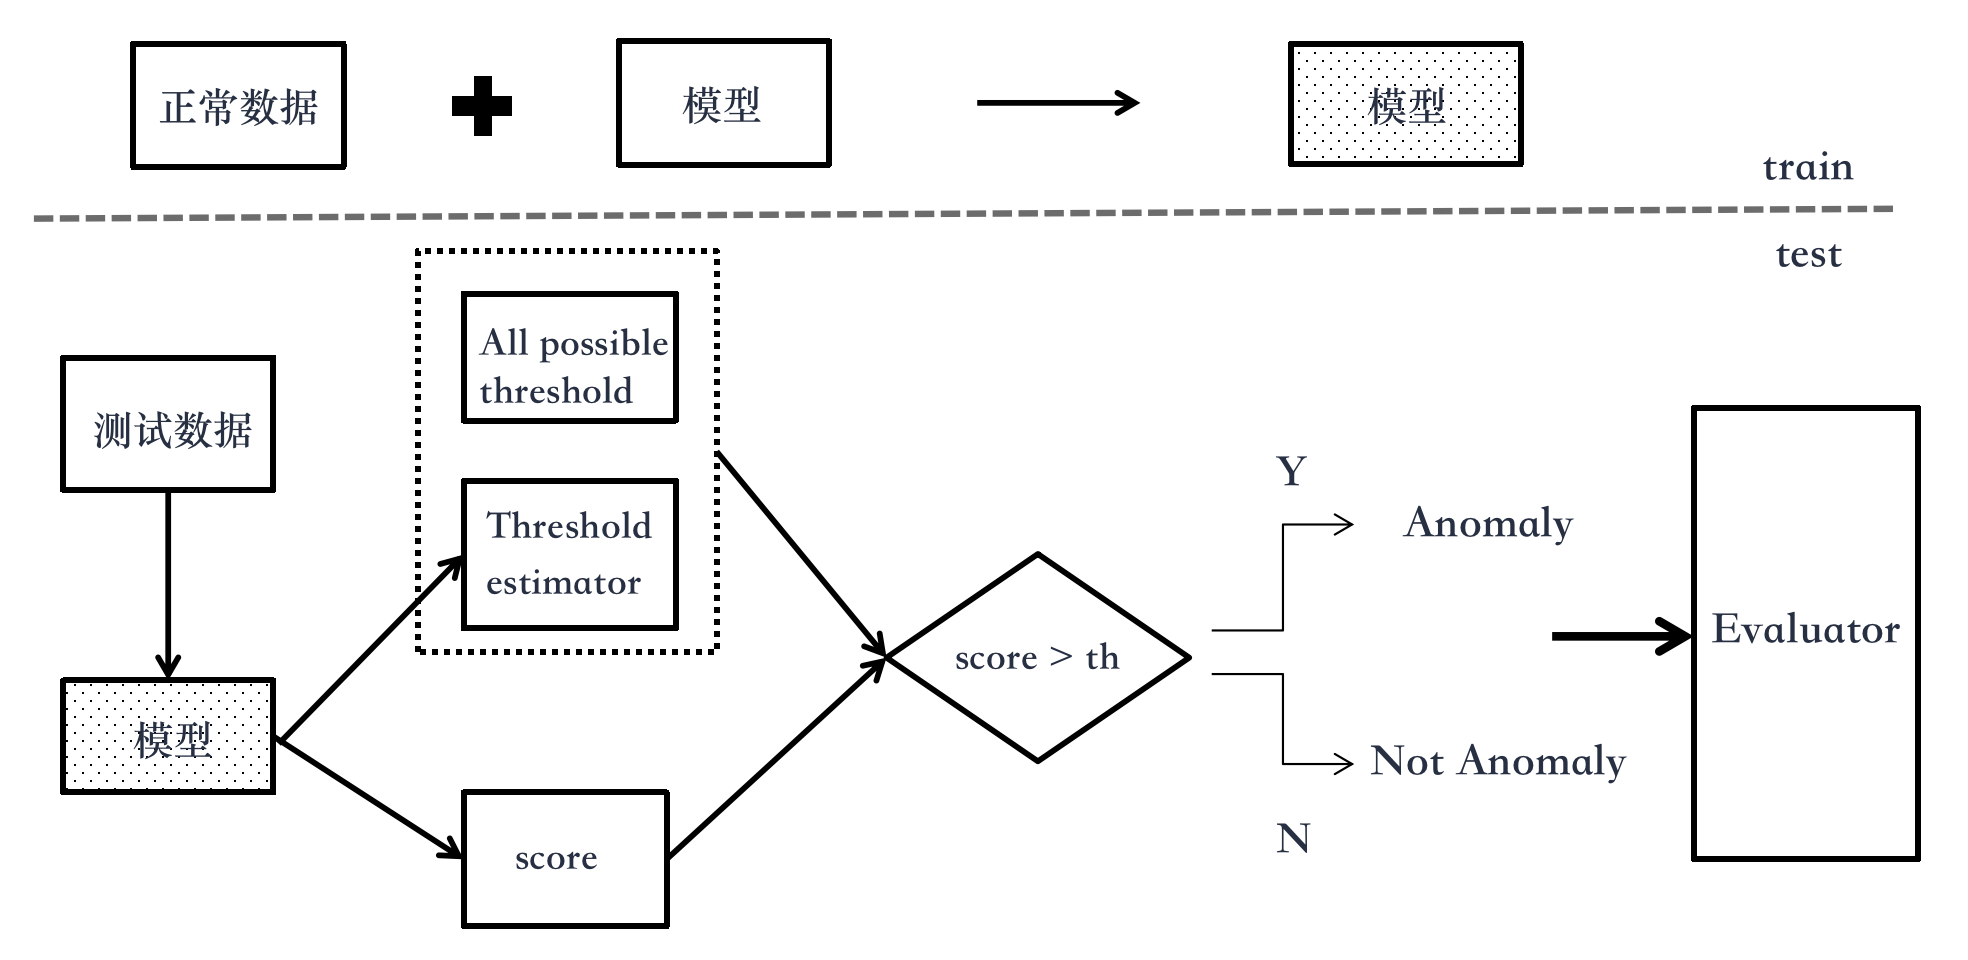
\includegraphics[width=\textwidth]{part1_overview.png}
    \caption{基于深度学习的时间序列异常检测框架}
    \label{fig:part1_overview}
  \end{figure}

我们的框架分为训练和测试两种运行模式。

在训练模式中,我们需要先用正常数据结合某个特定的模型训练出一个适用于该数据集的模型。然后在测试模式中时,模型对于每条数据会输出一个异常分数表示它的异常程度,通常情况下我们还需要模型来提供一个阈值,当异常程度>给定阈值时,认为该条数据是异常,否则认为正常,然后送到评估模块进行评估结果,或者我们枚举所有可能的阈值对结果进行评估,这样可以衡量模型的上限。

接下来分别对系统的几个关键部分进行阐述。

\section{数据集选择}
我们选择了在SMD(Server Machine Dataset)\cite{su2019robust}数据集上完成实验。其是从国内某互联网公司的服务器上采集的长达5周的kpi真实指标进行脱敏处理后的结果。其测量了28台机器上的38个指标长达5周的结果,也就是$M=38$,然后将数据平均分为了两部分,一部分全是正常数据不包含异常${\rm x}_{train}$,而另一部分则包含异常${\rm x}_test$并且提供了标记$y_{test}$用来测试。考虑到该数据格式符合我们云网络的场景,所以选择了该数据集。

\section{算法选择模块}
在算法的选择方面,本文实现了两部分的算法,一部分是复现一些经典的算法,另一部分则是对已有算法进行一些修改来适应于当前的问题。
\subsection{复现算法}
本文复现了一些经典的异常检测算法,主要包含两类,一类是用于单点异常检测的算法,即将每个时间点的数据当成独立不相关的数据进行检测,也就是将这些模型看做一个函数的话,就是$y_t = \phi ({\rm x}_t)$,例如AutoEncoder、Variational AutoEncoder\cite{an2015variational}、Deep SVDD\cite{ruff2018deep}、DAGMM\cite{zong2018deep}、ConAD\cite{nguyen2018anomaly};另一类则是判断每一时刻的状态时不仅要看当前的指标监测值,还要看之前一段时间数据,不妨令这段时间长度为$T$,则$y_t = \phi({\rm x}_{t-T},{\rm x}_{t-T+1},\dots,{\rm x}_{t})$,具体LSTM、LSTM-ED\cite{malhotra2016lstm}。
\subsection{改进算法}
在已有算法的基础上,我们做出了两方面的改进。

一方面是修改已有的用于单点异常检测的算法结构来使其适应时间序列异常检测,主要方法是将原算法中的Linear层替换成LSTM层来保留和捕捉历史信息,比方说对AutoEncoder的模型改变如图~\ref{fig:lstm_ae}所示。依据此种方法,我们对VAE、DAGMM、ConAD进行修改分别得到了LSTM-VAE、LSTM-DAGMM和LSTM-ConAD模型。
s
\begin{figure}[htbp]
  \begin{minipage}[t]{0.5\linewidth}
  \centering
  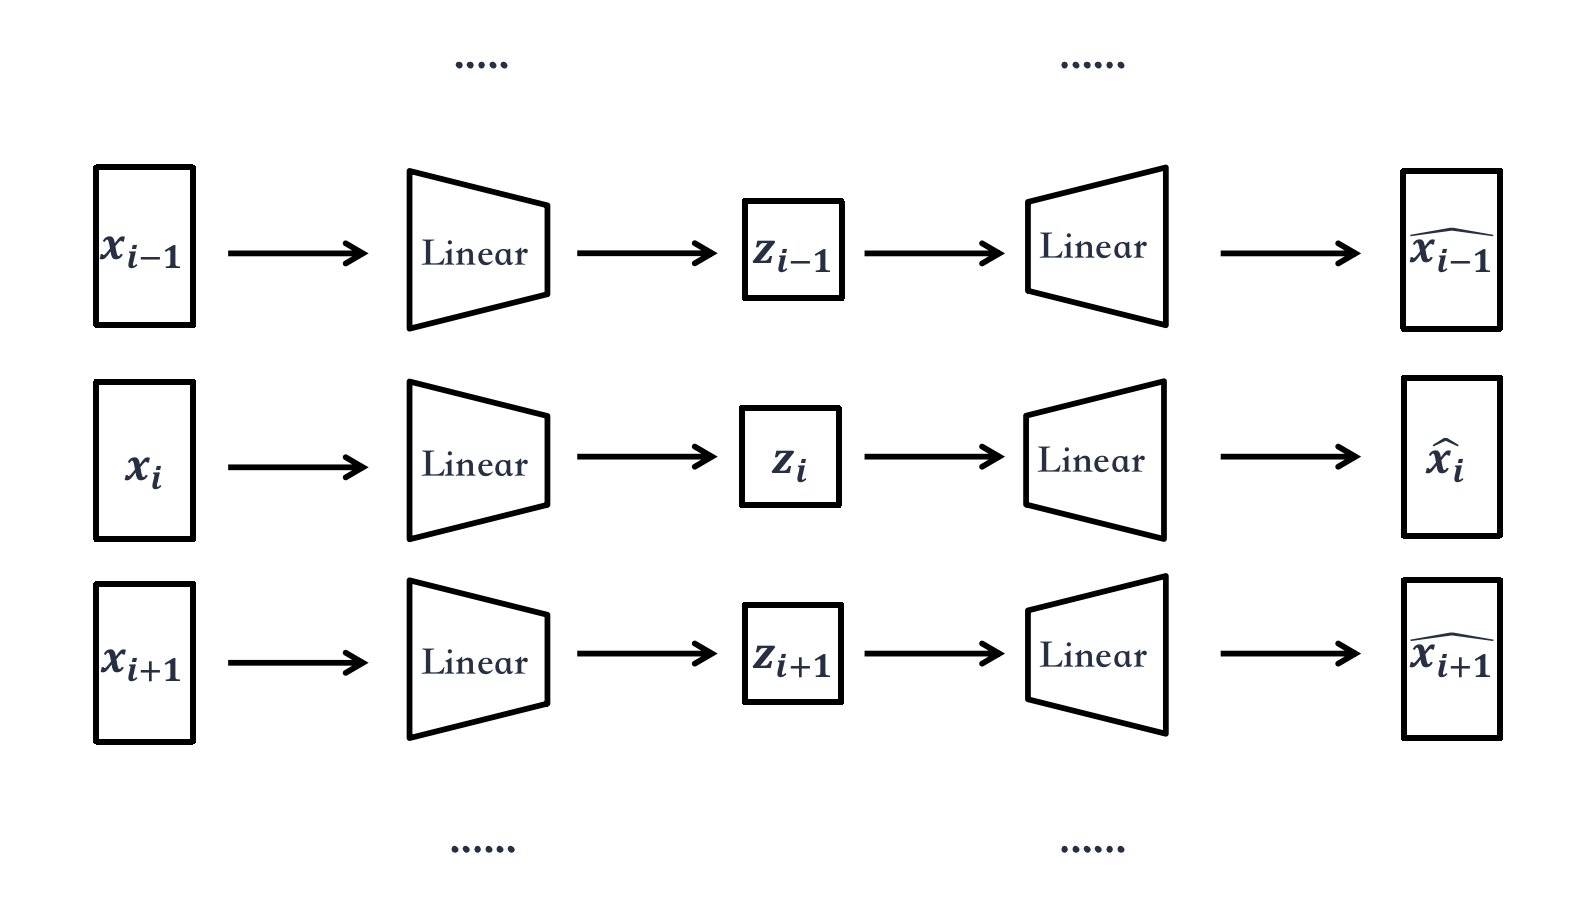
\includegraphics[width=\textwidth]{AE.png}
  \caption*{原先的AutoEncoder模型}
  \end{minipage}
  \begin{minipage}[t]{0.5\linewidth}
  \centering
  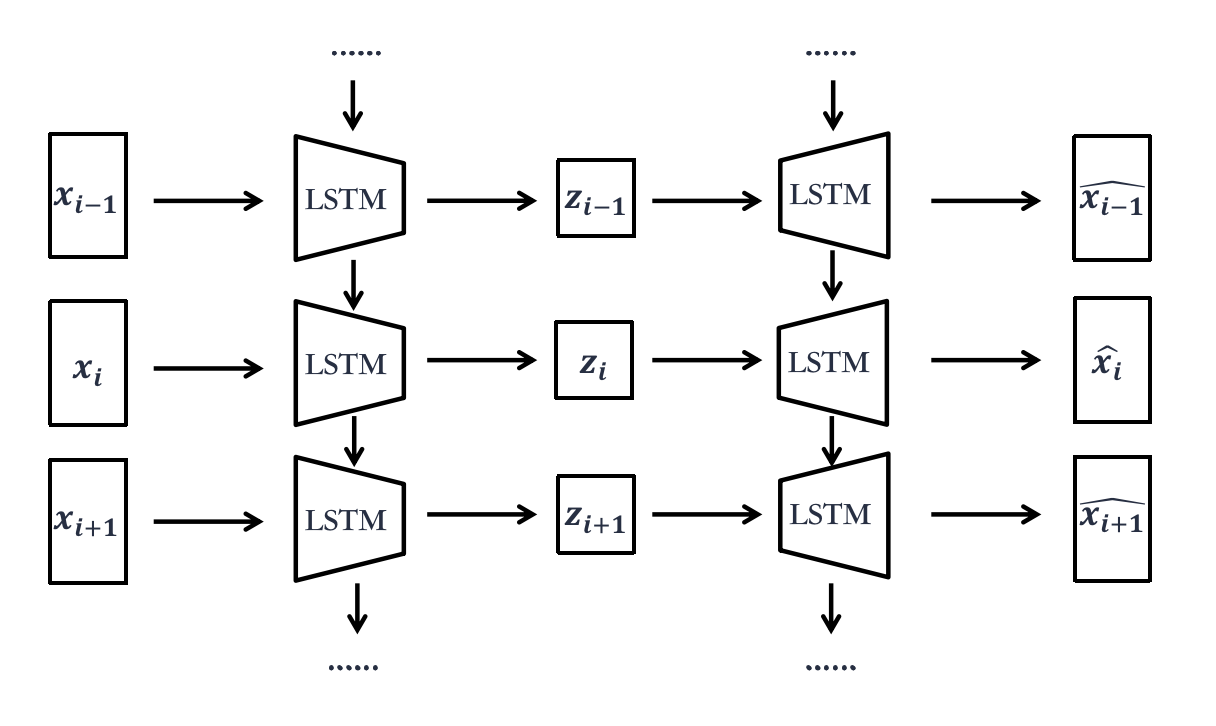
\includegraphics[width=0.95\textwidth]{LSTM_AE.png}
  \caption*{经过修改后的LSTM\_AE模型}
  \end{minipage}
  \caption{对AutoEncoder的模型修改过程}
  \label{fig:lstm_ae}
\end{figure}

另一方面是我们将LSTM的预测与AE的重构结合起来,提出了一个AE\_Predictor模型,其结构如图~\ref{fig:AE_Predictor}所示。

\begin{figure}[htbp]
  \centering
  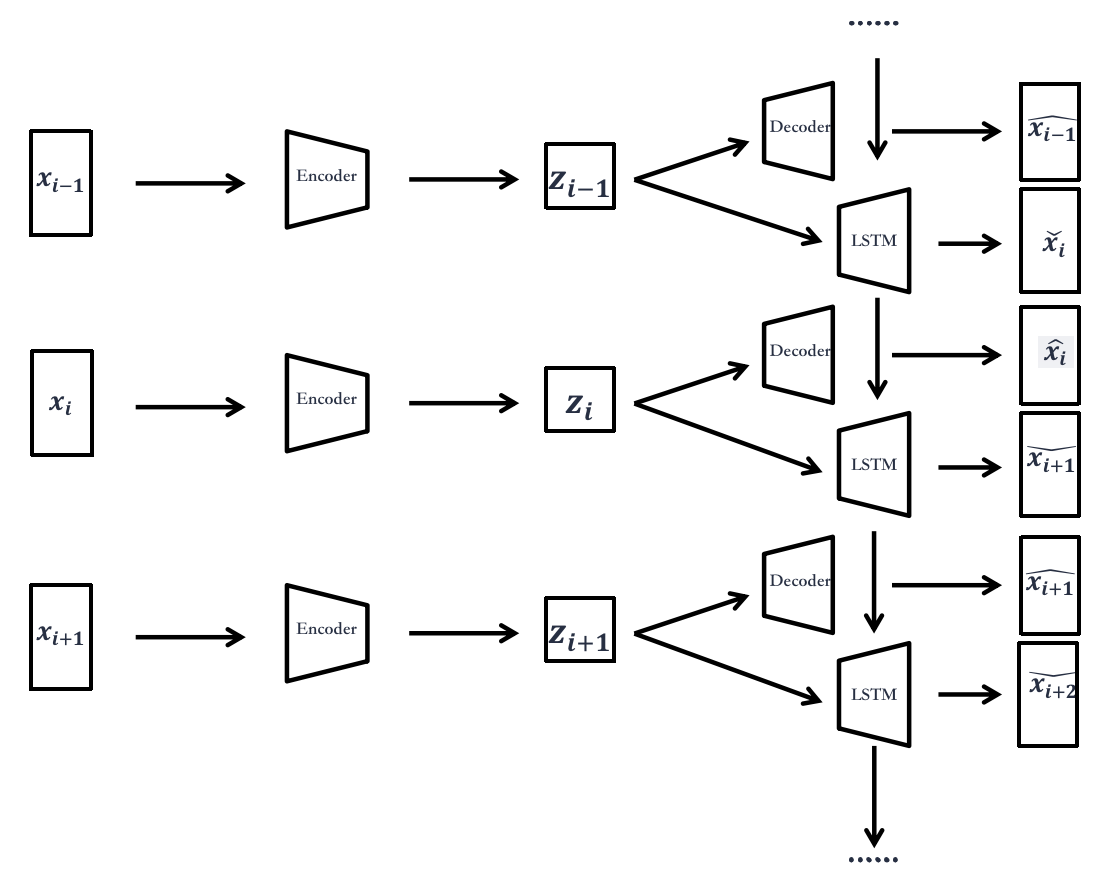
\includegraphics[width=\textwidth]{AE_Predictor.png}
  \caption{AE\_Predictor模型示意图}
  \label{fig:AE_Predictor}
\end{figure}

目的是要让AE学习的低维表示不仅具有重构当前数据的能力,同时低维表示序列还具有能够预测下一时刻数据的能力,也就是捕捉到时序依赖,以此达到更好的异常检测效果。

\section{动态阈值选取模块}
因为我们在算法选择部分均是实现的无监督的算法,因此通常算法输出的是一个异常分数的非负实数值,而不是一个0或者1的确切值,也就是说我们得到的实际是$s = [s_1, s_2,\dots,s_N]$,其中$s_t\in R^+$,$t\leq N$,要想进一步得到$y$,我们需要一个模型提供的或者人为提供的阈值threshold来作进一步的变换:
\begin{equation}
  y_t = \begin{cases}
    0, & s_t < threshold \cr
    1, & s_t \geq threshold
  \end{cases}
\end{equation}
通常情况下,该阈值的确立有多种方法,一种是假设异常分数满足特定分布,最常见的是高斯分布,但实际的异常分数很难从理论上证明符合高斯分布,通常情况下也确实不符合;一种是假设异常是异常分数最高的那一批,通过人为设定一个分位数,但这个分位数也可能不符合实际分布情况,而且,这两种方法都需要我们事先遍历整个测试集的情况下才能确立阈值,也就是我们要知道一条曲线的全貌之后才能确立它在之前的某个时刻是否异常,这在投入使用的时候是致命的,意味着异常检测极大的延迟,同时无法支持在线;还有一种方法是将测试集划分为验证集和测试集(因为测试集是有标的,验证集也是有标的,所以只能从原来的测试集中划分出验证集),通过在验证集上选取合适的阈值以及基于验证集和测试集情况类似的假设来期待在测试集上获得较好的效果。

受到\cite{siffer2017anomaly}的启发,我们使用了基于极值理论的方法来自动确立动态的阈值。

极值理论的好处是不会对数据的分布作任何假设,而Peak-Over-Threshold(POT)是极值理论的第二定理。POT的基本思想就是通过带有参数的广义Pareto分布(GPD)来拟合概率分布的尾部。我们的GPD函数如下:
\begin{equation}
  F(s) = P(th - S > s | S < th) \approx (1 + \frac{\gamma s}{\beta})^{-\frac{1}{\gamma}}
\end{equation}
其中$th$是异常分数的初始阈值,$\gamma$和$\beta$是GPD的形状和比例参数,S是{S1,S2,...,SN'}中的任何值。 低于阈值$th$的部分表示为$th-S$,并根据经验将其设置为低分位数。 与[22]类似,我们用最大似然估计的参数γˆ和β的最大值
(MLE)。 然后通过以下公式计算最终阈值thF:
\begin{equation}
  th_F \approx th - \frac{\hat{\beta}}{\hat{\gamma}}((\frac{qN'}{N'_{th}})^{-\hat{\gamma}}-1)
\end{equation}
其中q是观察S <th的期望概率,N次观察,N'是Si s.t的数目。 Si <th
日
对于POT方法,仅需要调整两个参数(低分位数和q)。 这两个参数在整个模型范围内,可以凭经验进行设置:低分位数(例如,小于7%)和q(例如10-4)\cite{siffer2017anomaly}。

当然,为了进一步衡量模型的上限,我们同样也会枚举所有可能的阈值,送到评估模块中获得结果最好的,作为模型上限的一个衡量标准。

\section{评价模块}
在异常检测领域,用的最多的评价指标是F\_1-Score,计算方式为
\begin{equation}
  Precision = \frac{TP}{TP + NP}
\end{equation}

\begin{equation}
  Recall = \frac{TP}{TP + FN}
\end{equation}

\begin{equation}
  F_1-Score = 2\times \frac { Precision \times Recall}{Precision + Recall}
\end{equation}
其中$TP、TN、FP、FN$分别代表true positives、true negatives、false positives、false negatives。$Precision$描绘的是实际异常占检测出的所有异常的比例,而$Recall$描绘了所有的异常中被检测到的比例,直觉上来看,两者是对立的,单用其中一个用来评价检测器的性能是不合理的。但在单点的异常检测中,将它们结合在一起的$F_1-Score$已经被认为是公认的有效的评价方式。但对于时间序列数据的异常检测来说,这样的评价就不太准确。主要原因是因为在时间序列数据中异常的发生通常是连续的一段,如图\ref{fig:anomaly_example}所示。我们使用的评价体系应该尽可能贴近实际投入使用的体验。对于一段真正的异常而言,不仅要考虑检测为异常的点的个数、还要考虑检测出来的位置。之前的一些工作\cite{xu2018unsupervised}\cite{su2019robust}用了一种point-wise的方法来对算法得到的结果进行调整然后再进行评估,具体就是对于一个真实的异常而言,如果我们的算法主要检测到了范围内的一个,那么整段异常就认为都被检测到。该评价方法没有考虑到检测到的点的位置和检测到的点数的影响,会造成评价指标的虚高。

基于以上考虑,我们借用了\cite{tatbul2018precision}的新型的Precision和Recall的计算方式。

首先我们将异常表示成区间的集合,真实的异常为$R=[R_1,R_2,\dots,R_{N_r}]$,其中每个$R_i$代表一个区间的异常,我们不放人为$R_i.l$和$R_i.r$分别代表该区间的左右端点。同理$P=[P_1,P_2,\dots,P_{N_p}]$表示预测出来的异常。
\begin{equation}
  Recall(R,P) = \frac{\sum_{i=1}^{N_r} Recall_T(R_i,P)}{N_r}
\end{equation}
其中$Recall_T$的计算由两部分加权组成:分别考虑了存在性以及位置性。
\begin{equation}
  Recall_T(R_i,P) = \alpha \times ExistenceReward(R_i,P) + (1-\alpha) \times OverlapReward (R_i,P)
\end{equation}
存在性只需要判断是否存在一个检测出的异常区间当前的实际异常有交集。
\begin{equation}
ExistenceReward(R_i,P) = \begin{cases} 1, & \ \exists \  | R_i \cap P_j|>1 \cr 0, & otherwise \end{cases}
\end{equation}
而相交性则需要考虑重叠的位置和大小的关系,此处我们认为对于一个异常来说,越开始检测到对我们来说越重要,因此我们将靠前的位置分配较大的权重,具体计算如图~\ref{algorithm:omega1}所示。
\begin{equation}
  OverlapReward(R_i,P) = \sum_{j=1}^{N_p}\omega(R_i,R_i\cap P_j)
\end{equation}
\begin{algorithm}
  \caption{$\omega$ 计算方法1}
  \begin{algorithmic}
      \Function{$\omega$}{AnomalyRange, OverlapRange}
      \State DetectValue \gets 0
      \State TotalValue \gets 0
      \State len \gets length(AnomalyRange)
      \For {i = 1  \to len}
          \State Value \gets len - i + 1
          \State TotalValue \gets TotalValue + Value
          \If {AnomalyRange[i] in OverlapRange}
              \State DetectValue \gets DetectValue + Value
          \EndIf
      \EndFor
      \State \Return $\frac{DetectValue}{TotalValue}$
      \EndFunction
  \end{algorithmic}
  \label{algorithm:omega1}
\end{algorithm}
意识到OverlapRange也一定是一个区间之后,我们可以将$\omega$的计算方式简化为如下:
  \begin{algorithm}
    \caption{$\omega$ 计算方法2}
    \begin{algorithmic}
        \Function{$\omega$}{AnomalyRange, OverlapRange}
        \State len \gets length(AnomalyRange)
        \State TotalValue \gets $\frac{len \times (len + 1)}{2}$
        \State l \gets OverlapRange.l - AnomalyRange.l + 1
        \State r \gets OverlapRange.r - AnomalyRange.l + 1
        \State DetectValue \gets $\frac{r \times (r+1)}{2} - \frac{(l-1) \times l}{2}$
        \State \Return $\frac{DetectValue}{TotalValue}$
        \EndFunction
    \end{algorithmic}
    \label{algorithm:omega2}
  \end{algorithm}

新型Precision的计算方式类似:

\begin{equation}
Precision(R,P) = \frac{\sum_{i=1}^{N_p}Precision_T(R,P_i)}{N_p}
\end{equation}

区别是$Precision_t(R,P_i)$的计算不需要考虑$ExistenceReward$,直接按照检测到的位置算贡献即可:
\begin{equation}
Precision_T(R,P_i) = \sum_{j=1}^{N_r}\omega(P_i,P_i\cap R_j)
\end{equation}


  该评价方式虽然考虑的全面,但是随之而来的就是计算代价很大,复杂度为$O(N_r\times N_p)$。当我们需要计算所有阈值的结果并选取最好的时候,考虑阈值按从大到小枚举所有可能的$N$个,最坏情况下的$N_p$序列为$\{1,2,3,\dots,\frac{N}{2},\frac{N}{2}-1,\frac{N}{2}-2,\dots,1\}$,则总的计算复杂度为$O(N_r\times N^2)$。

  \begin{algorithm}
  \caption{朴素的Best F1-Score计算方式}
  \begin{algorithmic}[1]
    \Require TAT
    \Ensure 最好的F1-Score
    \Function {computeBestF1Score}{R,S}
    \State bestF1Score = 0
    \ForAll {$s \in S$}
    \State P \gets translateTo01(S,s)
    \State bestF1Score \gets max(bestF1Score, computeF1Score(R,P))
    \EndFor
    \State \Return bestF1Score
    \EndFunction
  \end{algorithmic}
  \end{algorithm}


  我们考虑一种新的增量计算的方式,每次将阈值下调时,考虑只有一个位置$i$的预测结果从0变成了1,那么有可能有三种情况:
  \begin{enumerate}
    \item 这一个位置形成了一个新的异常区间,也就是$i-1$和$i+1$都是不存在或者为0的状态
    \item 这个位置拓宽了相邻的区间,也就是$i-1$或者$i+1$中有且只有一个位置已经被预测为1
    \item 这个位置将左右两个区间连成了一个区间,也就是$i-1$与$i+1$都存在且被预测为异常
  \end{enumerate}

  如果我们能够以一个较低的复杂度支持动态的在$P$中增加、减少一个异常区间同时计算Precision和Recall的值,那么就能高效的求解best F1-Score。具体来讲,我们通过记录中间变量的方式来记录计算过程中的中间状态,通过并查集的方式来快速维护$P$。具体的算法过程如下:

  \begin{breakablealgorithm}
    \caption{高效的Best F1-Score计算方式}
    \begin{algorithmic}[1]
      \Require TAT
      \Ensure 最好的F1-Score
      \State $rangeReward \gets [0] * N_r$
      \State $rangeOverlapCount \gets [0] * N_r$
      \State $Recall \gets 0$
      \State $Precision \gets 0$

      \State

      \Function {computeBestF1Score}{R,S}
      \State bestF1Score = 0
      \State S \gets sorted(S) in descending order
      \ForAll {$s \in S$}
      \State i \gets indexOf(s)
      \State predict[i] = 1
      \If { $i + 1 < n and predict[i + 1] = 1$}
          \State \Call{dropPredictRange}{getRange(i + 1)}
          \State \Call{union}{i, i + 1}
      \EndIf
      \If {$i - 1 \geq 0 and predict[i - 1] = 1$}:
          \State \Call{dropPredictRange}{(getRange(i - 1)}
          \State \Call{union}{i, i - 1}
      \EndIf
      \Call{addPredictRange}{getRange(i)}
      \State $bestF1Score \gets max(bestF1Score, 2\times\frac{Precision \times Recall}{Precision + Recall})$
      \EndFor
      \State \Return bestF1Score
      \EndFunction
      
      \State

      \Function {addPredictRange}{p}
      \State Recall \gets 0
      \ForAll $R_i \in R$
            \State $rangeReward_i += \omega(R_i,R_i \cap p)$
            \State $overlapCount_i += |R_i\cap p|$
            \If {$overlapCount_i > 0$}
              \State existReward = 1
            \Else
              \State existReward = 0
            \EndIf
            \State $overlapReward \gets rangeReward_i$
            \State $Recall += \alpha \times existReward + (1-\alpha) \times overlapReward$
      \EndFor
      \State $Recall /= N_r$

      \State

      \State reward \gets 0
      \ForAll $R_i \in R$
            \State $reward += \omega(p, p \cap R_i)$
      \EndFor
      \State $Precision \gets \frac{Precision \times N_p + reward}{N_p + 1}$
      \State $N_p += 1$
      \EndFunction

      \State

      \Function {dropPredictRange}{p}
      \State Recall \gets 0
      \ForAll $R_i \in R$
            \State $rangeReward_i -= \omega(R_i,R_i \cap p)$
            \State $overlapCount_i -= |R_i\cap p|$
            \If {$overlapCount_i > 0$}
              \State existReward = 1
            \Else
              \State existReward = 0
            \EndIf
            \State $overlapReward \gets rangeReward_i$
            \State $Recall += \alpha \times existReward + (1-\alpha) \times overlapReward$
      \EndFor

      \State

      \State $Recall /= N_r$

      \State reward \gets 0
      \ForAll $R_i \in R$
            \State $reward += \omega(p, p \cap R_i)$
      \EndFor
      \State $Precision \gets \frac{Precision \times N_p - reward}{N_p - 1}$
      \State $N_p -= 1$
      \EndFunction
    \end{algorithmic}
  \end{breakablealgorithm}
  其中getRange和Union是通过并查集来实现记录和维护某个位置所属的区间以及该区间的左右端点,算法中不再赘述。容易得知这样的计算复杂度为$O(N_r\times N)$,较原先下降了一个数量级,实测原先需要4小时的计算仅需3秒就可以得出结果。
\section{实验结果与分析}
我们考虑实验结果主要从三方面来分析,一方面是各个模型在best F1-Score上的表现,也就是模型上限的衡量。再一方面,我们考虑各个模型在用POT确立阈值之后的表现,最后,我们还要关注各个模型的效率问题,尤其是测试阶段的效率,因为这影响到我们模型的上限。

在best F1-Score上的表现,各个模型的结果如表所示,其中各个指标的计算方式是由28台机器的结果取平均得到。除了本文实现的模型外,我们还加入了当前state-of-the-art的工作OminiAnomaly\cite{su2019robust}的输出结果来评价,方便做对比。

我们可以看到OmniAnomaly在我们的框架下表现并不突出,可能是的因为原先的评价标准错误地表示了模型的能力。此外,我们还可以看到,表现的较好。

在POT F1-Score上的表现,各个模型的结果如表所示,

该部分结果与best 结果类似,best F1-Score比较好的,POT的方法的出来的指标也不会差。所以我们可以认为best F1-Score还是有一定的说服力;另一方面,大部分算法在使用POT之后效率下降地都比较明显,所以POT方法捕捉模型上限的能力还待商榷;最后,我们在测试时观察到POT的两个超参选取会较大地影响到模型的结果,所以POT的方法结果还是不够鲁棒。

在时间效率上,各个算法的结果如下,,可以看出,综合效果和速率,如果投入使用的话,xx算法是个不错的选择。



